\documentclass[tikz,border=10pt]{standalone}
\usepackage{tikz}
\usetikzlibrary{
  shapes.geometric,
  arrows.meta, arrows,
  positioning, fit, backgrounds,
  shadows, matrix, calc
}

\tikzset{
  hwnode/.style={rectangle,rounded corners=4pt,fill=yellow!40,draw=orange!70,
    text width=2.0cm,align=center,minimum height=0.9cm,font=\small\bfseries,drop shadow},
  srvnode/.style={rectangle,rounded corners=4pt,fill=green!25,draw=green!60!black,
    text width=2.4cm,align=center,minimum height=0.9cm,font=\small\bfseries,drop shadow},
  dbnode/.style={cylinder,shape border rotate=90,fill=blue!25,draw=blue!60,
    text width=1.8cm,align=center,minimum height=1.1cm,font=\small\bfseries},
  uinode/.style={rectangle,rounded corners=4pt,fill=purple!20,draw=purple!60,
    text width=2.2cm,align=center,minimum height=0.9cm,font=\small\bfseries,drop shadow},
  queuenode/.style={rectangle,rounded corners=4pt,fill=orange!25,draw=orange!60,
    text width=2.0cm,align=center,minimum height=0.85cm,font=\small\bfseries},
  arr/.style={-{Stealth[length=6pt]},thick,draw=gray!60}
}

\begin{document}

%% ============================================================
%% DIAGRAM 1 — System Architecture
%% ============================================================
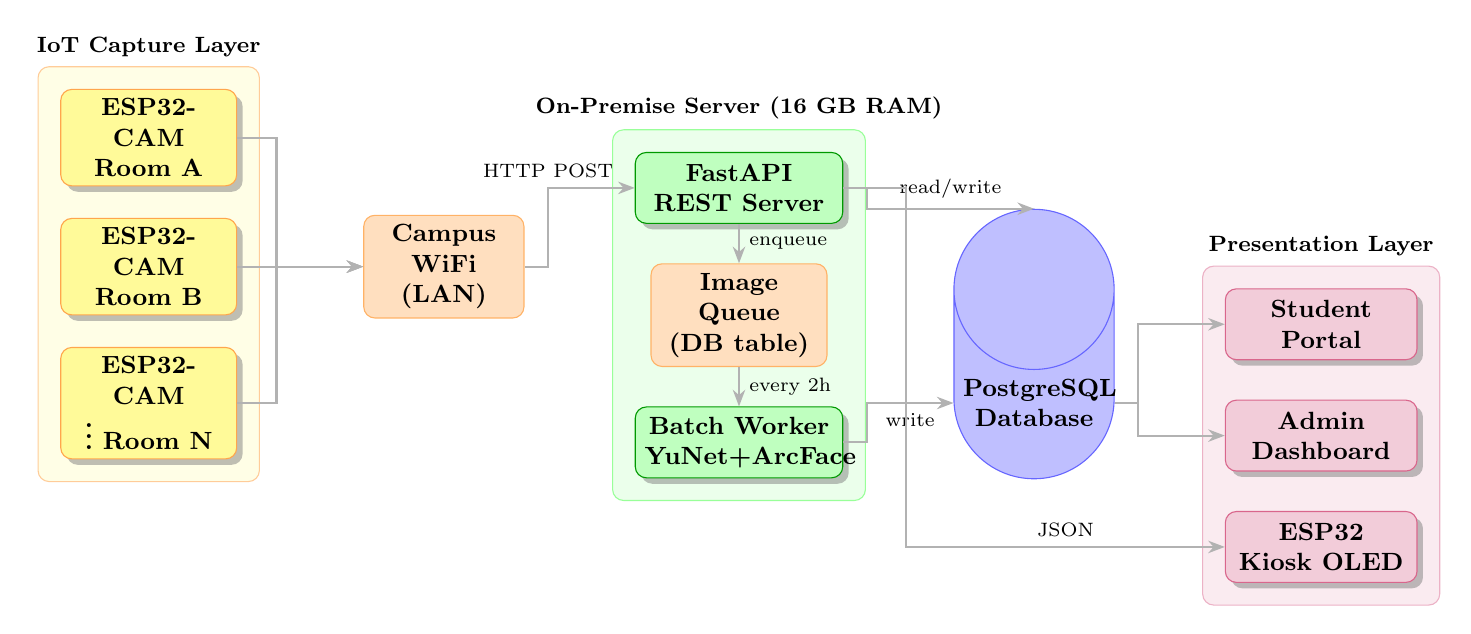
\begin{tikzpicture}[node distance=1.0cm and 1.4cm]

  % IoT Layer
  \node[hwnode] (esp1) {ESP32-CAM\\Room A};
  \node[hwnode,below=0.4cm of esp1] (esp2) {ESP32-CAM\\Room B};
  \node[hwnode,below=0.4cm of esp2] (espN) {ESP32-CAM\\$\vdots$ Room N};

  \begin{scope}[on background layer]
    \node[fit=(esp1)(esp2)(espN),fill=yellow!10,draw=orange!40,rounded corners,
      label={[font=\footnotesize\bfseries]above:IoT Capture Layer},inner sep=8pt] (iot) {};
  \end{scope}

  % WiFi
  \node[queuenode,right=1.6cm of esp2,text width=1.8cm,minimum height=0.7cm]
    (wifi) {Campus\\WiFi (LAN)};

  \draw[arr] (esp1.east) -- ++(0.5,0) |- (wifi.west);
  \draw[arr] (esp2.east) -- (wifi.west);
  \draw[arr] (espN.east) -- ++(0.5,0) |- (wifi.west);

  % Server components
  \node[srvnode,right=1.4cm of wifi,yshift=1.0cm] (api) {FastAPI\\REST Server};
  \node[queuenode,below=0.5cm of api] (queue) {Image Queue\\(DB table)};
  \node[srvnode,below=0.5cm of queue] (worker) {Batch Worker\\YuNet+ArcFace};

  \draw[arr] (wifi.east) -- ++(0.3,0) |- (api.west) node[midway,above,font=\scriptsize]{HTTP POST};
  \draw[arr] (api) -- (queue) node[midway,right,font=\scriptsize]{enqueue};
  \draw[arr] (queue) -- (worker) node[midway,right,font=\scriptsize]{every 2h};

  \begin{scope}[on background layer]
    \node[fit=(api)(queue)(worker),fill=green!8,draw=green!40,rounded corners,
      label={[font=\footnotesize\bfseries]above:On-Premise Server (16 GB RAM)},inner sep=8pt] (srv) {};
  \end{scope}

  % Database
  \node[dbnode,right=1.4cm of worker,yshift=0.5cm] (db) {PostgreSQL\\Database};
  \draw[arr] (worker.east) -- ++(0.3,0) |- (db.west) node[near end,below,font=\scriptsize]{write};
  \draw[arr] (api.east) -- ++(0.3,0) |- (db.north) node[near end,above,font=\scriptsize]{read/write};

  % Dashboards
  \node[uinode,right=1.4cm of db,yshift=1.0cm] (stud) {Student\\Portal};
  \node[uinode,below=0.5cm of stud] (admin) {Admin\\Dashboard};
  \node[uinode,below=0.5cm of admin] (kiosk) {ESP32\\Kiosk OLED};

  \draw[arr] (db.east) -- ++(0.3,0) |- (stud.west);
  \draw[arr] (db.east) -- ++(0.3,0) |- (admin.west);
  \draw[arr] (api.east) -- ++(0.8,0) |- (kiosk.west) node[near end,font=\scriptsize,above]{JSON};

  \begin{scope}[on background layer]
    \node[fit=(stud)(admin)(kiosk),fill=purple!8,draw=purple!30,rounded corners,
      label={[font=\footnotesize\bfseries]above:Presentation Layer},inner sep=8pt] {};
  \end{scope}

\end{tikzpicture}

%% ============================================================
%% DIAGRAM 2 — Batch Processing Pipeline
%% ============================================================
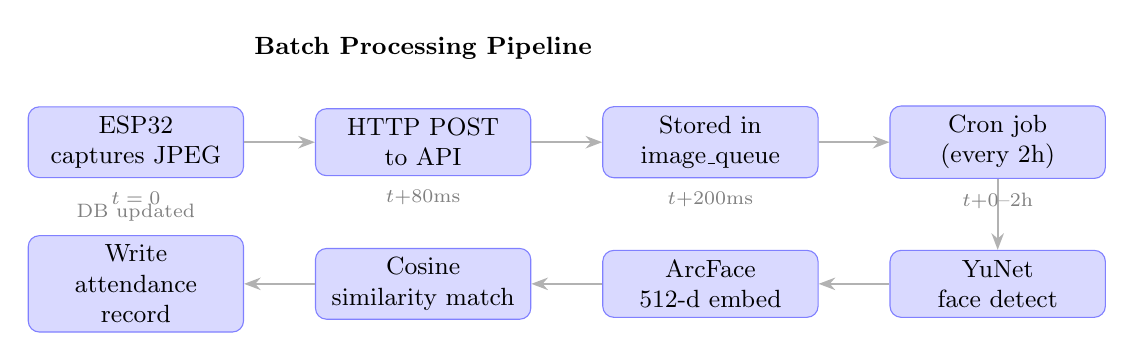
\begin{tikzpicture}[node distance=0.7cm and 0.9cm,
  pstep/.style={rectangle,rounded corners=4pt,fill=blue!15,draw=blue!50,
    text width=2.5cm,align=center,minimum height=0.85cm,font=\small}]

  \node[pstep] (s1) {ESP32\\captures JPEG};
  \node[pstep,right=0.9cm of s1] (s2) {HTTP POST\\to API};
  \node[pstep,right=0.9cm of s2] (s3) {Stored in\\image\_queue};
  \node[pstep,right=0.9cm of s3] (s4) {Cron job\\(every 2h)};
  \node[pstep,below=0.9cm of s4] (s5) {YuNet\\face detect};
  \node[pstep,left=0.9cm of s5] (s6) {ArcFace\\512-d embed};
  \node[pstep,left=0.9cm of s6] (s7) {Cosine\\similarity match};
  \node[pstep,left=0.9cm of s7] (s8) {Write\\attendance\\record};

  \draw[arr] (s1)--(s2);
  \draw[arr] (s2)--(s3);
  \draw[arr] (s3)--(s4);
  \draw[arr] (s4)--(s5);
  \draw[arr] (s5)--(s6);
  \draw[arr] (s6)--(s7);
  \draw[arr] (s7)--(s8);

  \node[font=\scriptsize,text=gray,below=0.05cm of s1] {$t=0$};
  \node[font=\scriptsize,text=gray,below=0.05cm of s2] {$t{+}80$ms};
  \node[font=\scriptsize,text=gray,below=0.05cm of s3] {$t{+}200$ms};
  \node[font=\scriptsize,text=gray,below=0.05cm of s4] {$t{+}0$--$2$h};
  \node[font=\scriptsize,text=gray,above=0.05cm of s8] {DB updated};

  % Label
  \node[font=\bfseries\small,above=0.5cm of s2] {Batch Processing Pipeline};

\end{tikzpicture}

%% ============================================================
%% DIAGRAM 3 — Database ER (simplified)
%% ============================================================
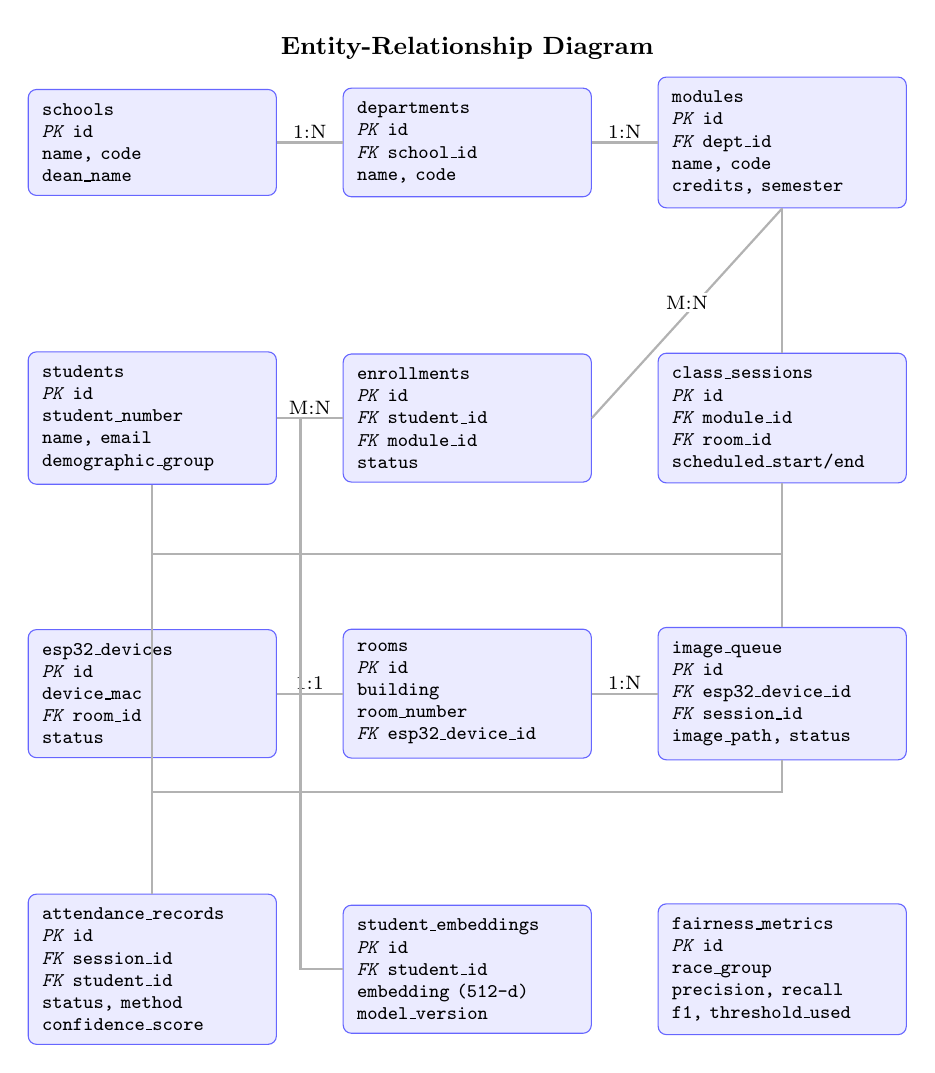
\begin{tikzpicture}[
  ent/.style={rectangle,draw=blue!60,fill=blue!8,rounded corners=3pt,
    font=\ttfamily\scriptsize,inner sep=5pt,text width=2.8cm,align=left},
  rel/.style={draw=gray!60,thick},
  lbl/.style={font=\scriptsize,fill=white,inner sep=1pt}
]

\node[ent] (schools) at (0,0) {
  \textbf{schools}\\
  \textit{PK} id\\
  name, code\\
  dean\_name
};
\node[ent] (depts) at (4,0) {
  \textbf{departments}\\
  \textit{PK} id\\
  \textit{FK} school\_id\\
  name, code
};
\node[ent] (modules) at (8,0) {
  \textbf{modules}\\
  \textit{PK} id\\
  \textit{FK} dept\_id\\
  name, code\\
  credits, semester
};
\node[ent] (students) at (0,-3.5) {
  \textbf{students}\\
  \textit{PK} id\\
  student\_number\\
  name, email\\
  demographic\_group
};
\node[ent] (enrollments) at (4,-3.5) {
  \textbf{enrollments}\\
  \textit{PK} id\\
  \textit{FK} student\_id\\
  \textit{FK} module\_id\\
  status
};
\node[ent] (sessions) at (8,-3.5) {
  \textbf{class\_sessions}\\
  \textit{PK} id\\
  \textit{FK} module\_id\\
  \textit{FK} room\_id\\
  scheduled\_start/end
};
\node[ent] (esp32) at (0,-7) {
  \textbf{esp32\_devices}\\
  \textit{PK} id\\
  device\_mac\\
  \textit{FK} room\_id\\
  status
};
\node[ent] (rooms) at (4,-7) {
  \textbf{rooms}\\
  \textit{PK} id\\
  building\\
  room\_number\\
  \textit{FK} esp32\_device\_id
};
\node[ent] (imgqueue) at (8,-7) {
  \textbf{image\_queue}\\
  \textit{PK} id\\
  \textit{FK} esp32\_device\_id\\
  \textit{FK} session\_id\\
  image\_path, status
};
\node[ent] (attendance) at (0,-10.5) {
  \textbf{attendance\_records}\\
  \textit{PK} id\\
  \textit{FK} session\_id\\
  \textit{FK} student\_id\\
  status, method\\
  confidence\_score
};
\node[ent] (embeddings) at (4,-10.5) {
  \textbf{student\_embeddings}\\
  \textit{PK} id\\
  \textit{FK} student\_id\\
  embedding (512-d)\\
  model\_version
};
\node[ent] (fairness) at (8,-10.5) {
  \textbf{fairness\_metrics}\\
  \textit{PK} id\\
  race\_group\\
  precision, recall\\
  f1, threshold\_used
};

% Relationships
\draw[rel] (schools.east) -- node[lbl,above]{1:N} (depts.west);
\draw[rel] (depts.east) -- node[lbl,above]{1:N} (modules.west);
\draw[rel] (students.east) -- node[lbl,above]{M:N} (enrollments.west);
\draw[rel] (enrollments.east) -- node[lbl,above]{M:N} (modules.south);
\draw[rel] (modules.south) -- ++(0,-0.5) -| (sessions.north);
\draw[rel] (sessions.south) -- (imgqueue.north);
\draw[rel] (esp32.east) -- node[lbl,above]{1:1} (rooms.west);
\draw[rel] (rooms.east) -- node[lbl,above]{1:N} (imgqueue.west);
\draw[rel] (imgqueue.south) -- ++(0,-0.4) -| (attendance.north);
\draw[rel] (sessions.south) -- ++(0,-0.9) -| (attendance.north);
\draw[rel] (students.south) -- (attendance.north);
\draw[rel] (students.east) -- ++(0.3,0) |- (embeddings.west);

% Title
\node[font=\bfseries\small] at (4,1.2) {Entity-Relationship Diagram};

\end{tikzpicture}

%% ============================================================
%% DIAGRAM 4 — ESP32 Kiosk Physical Unit
%% ============================================================
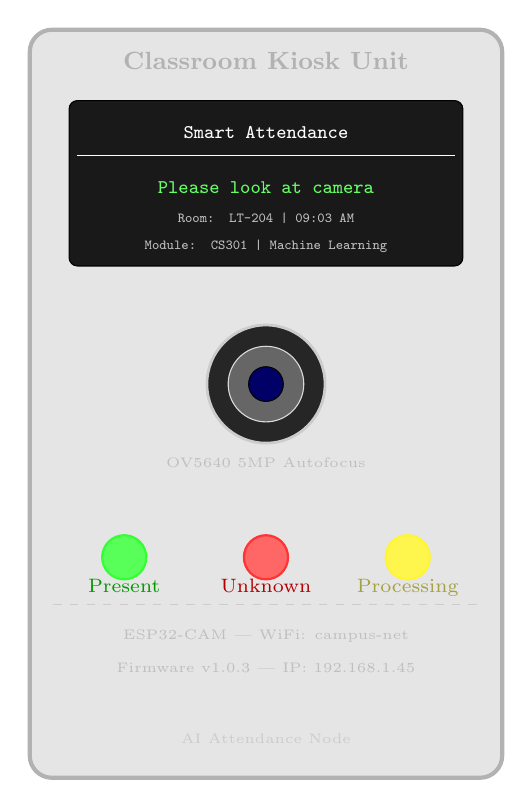
\begin{tikzpicture}

  % Enclosure
  \draw[rounded corners=8pt,fill=gray!20,draw=gray!60,line width=1.5pt]
    (0,0) rectangle (6,9.5);
  \node[font=\small\bfseries,text=gray!60] at (3,9.1) {Classroom Kiosk Unit};

  % OLED display
  \draw[fill=black!90,rounded corners=3pt] (0.5,6.5) rectangle (5.5,8.6);
  \node[font=\ttfamily\scriptsize,text=white] at (3,8.2) {\textbf{Smart Attendance}};
  \draw[white,thin] (0.6,7.9) -- (5.4,7.9);
  \node[font=\ttfamily\scriptsize,text=green!60] at (3,7.5) {Please look at camera};
  \node[font=\ttfamily\tiny,text=gray!50] at (3,7.1) {Room: LT-204  |  09:03 AM};
  \node[font=\ttfamily\tiny,text=gray!50] at (3,6.75) {Module: CS301 — Machine Learning};

  % Camera lens
  \draw[fill=black!85,draw=gray!40,line width=1pt] (3,5.0) circle (0.75cm);
  \draw[fill=black!60,draw=gray!30] (3,5.0) circle (0.48cm);
  \draw[fill=blue!40!black] (3,5.0) circle (0.22cm);
  \node[font=\tiny,text=gray!50] at (3,4.0) {OV5640 5MP Autofocus};

  % LEDs
  \draw[fill=green!65,draw=green!80,line width=0.8pt] (1.2,2.8) circle (0.28cm);
  \node[font=\scriptsize,below=0.15cm of {(1.2,2.8)}] {\textcolor{green!60!black}{Present}};

  \draw[fill=red!60,draw=red!80,line width=0.8pt] (3.0,2.8) circle (0.28cm);
  \node[font=\scriptsize,below=0.15cm of {(3.0,2.8)}] {\textcolor{red!70!black}{Unknown}};

  \draw[fill=yellow!70,draw=yellow!80,line width=0.8pt] (4.8,2.8) circle (0.28cm);
  \node[font=\scriptsize,below=0.15cm of {(4.8,2.8)}] {\textcolor{yellow!60!black}{Processing}};

  % Divider
  \draw[gray!40,dashed] (0.3,2.2) -- (5.7,2.2);
  \node[font=\tiny,text=gray!50] at (3,1.8) {ESP32-CAM  |  WiFi: campus-net};
  \node[font=\tiny,text=gray!50] at (3,1.4) {Firmware v1.0.3  |  IP: 192.168.1.45};
  \node[font=\tiny,text=gray!40] at (3,0.5) {AI Attendance Node};

\end{tikzpicture}

%% ============================================================
%% DIAGRAM 5 — Admin Dashboard Layout
%% ============================================================
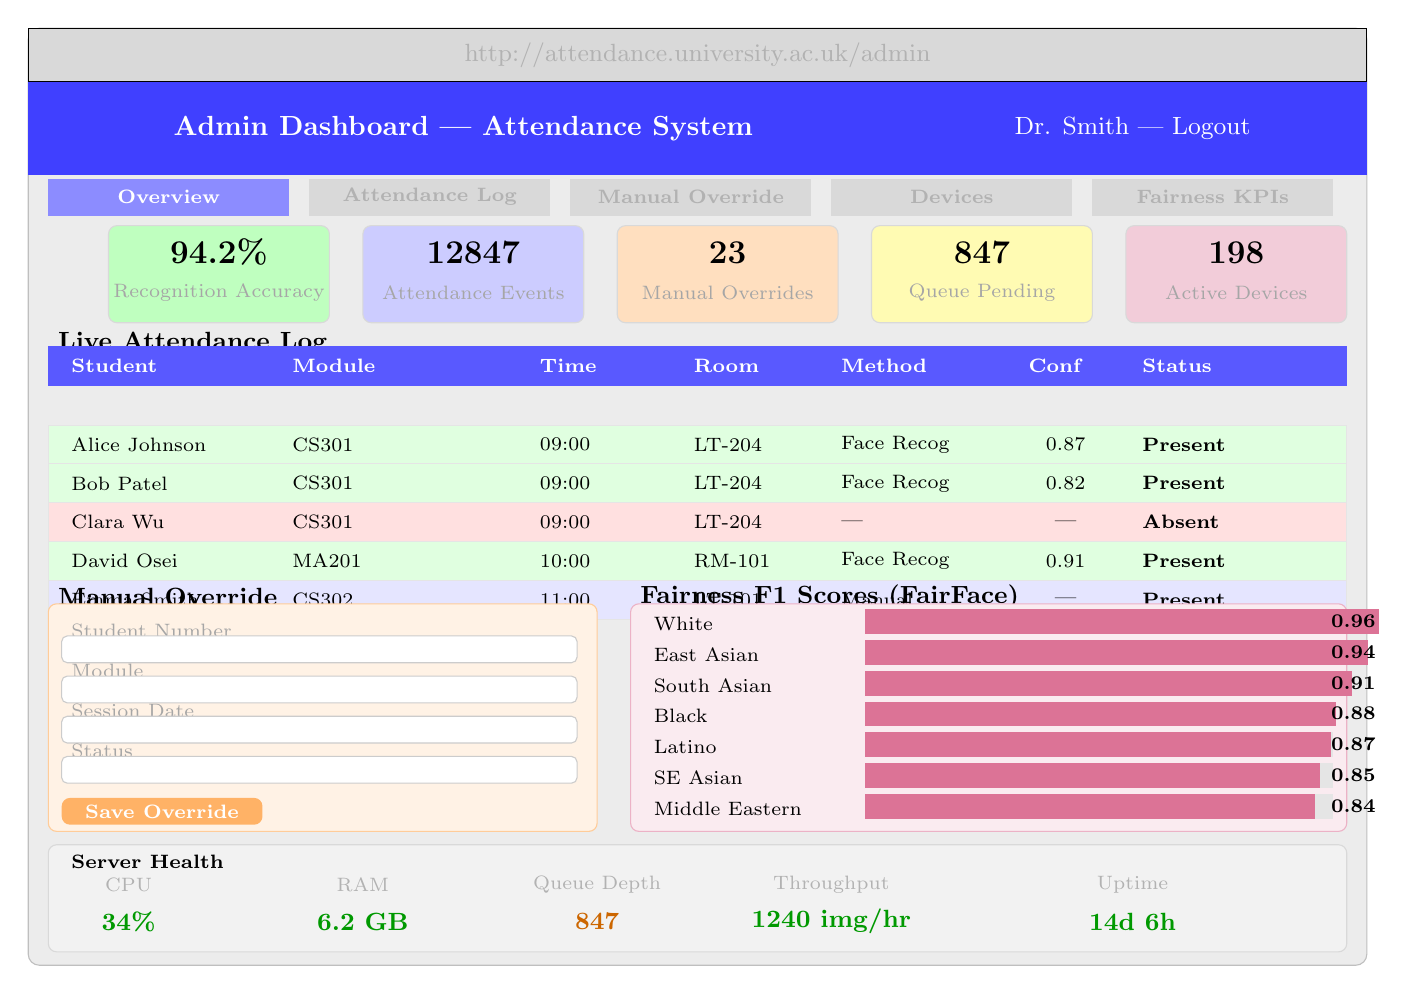
\begin{tikzpicture}[scale=0.85]

  % Browser frame
  \draw[fill=gray!15,draw=gray!50,rounded corners=4pt] (0,0) rectangle (20,14);
  \draw[fill=gray!30] (0,13.2) rectangle (20,14);
  \node[font=\small,text=gray!60] at (10,13.6) {http://attendance.university.ac.uk/admin};

  % Header bar
  \draw[fill=blue!75,draw=none] (0,11.8) rectangle (20,13.2);
  \node[font=\bfseries,text=white] at (6.5,12.5) {Admin Dashboard — Attendance System};
  \node[font=\small,text=white!80] at (16.5,12.5) {Dr. Smith  |  Logout};

  % Nav tabs — active tab drawn first, rest in loop
  \draw[fill=blue!45,draw=none] (0.3,11.2) rectangle (3.9,11.75);
  \node[font=\scriptsize\bfseries,text=white] at (2.1,11.48) {Overview};
  \foreach \i/\lbl in {1/{Attendance Log},2/{Manual Override},3/Devices,4/{Fairness KPIs}}{
    \pgfmathsetmacro{\xstart}{0.3+\i*3.9}
    \pgfmathsetmacro{\xend}{\xstart+3.6}
    \draw[fill=gray!30,draw=none] (\xstart,11.2) rectangle (\xend,11.75);
    \node[font=\scriptsize\bfseries,text=gray!60] at (\xstart+1.8,11.48) {\lbl};
  }

  % KPI cards
  \foreach \i/\val/\lbl/\col in {
    0/{94.2\%}/Recognition Accuracy/green!25,
    1/12847/Attendance Events/blue!20,
    2/23/Manual Overrides/orange!25,
    3/847/Queue Pending/yellow!30,
    4/198/Active Devices/purple!20
  }{
    \pgfmathsetmacro{\xc}{1.2+\i*3.8}
    \draw[fill=\col,draw=gray!30,rounded corners=3pt]
      (\xc,9.6) rectangle (\xc+3.3,11.05);
    \node[font=\large\bfseries] at (\xc+1.65,10.65) {\val};
    \node[font=\scriptsize,text=gray!70] at (\xc+1.65,10.05) {\lbl};
  }

  % Attendance log table header
  \node[font=\small\bfseries,anchor=west] at (0.3,9.3) {Live Attendance Log};
  \draw[fill=blue!65,draw=none] (0.3,8.65) rectangle (19.7,9.25);
  \foreach \x/\hdr in {0.5/Student,3.8/Module,7.5/Time,9.8/Room,12.0/Method,14.8/Conf,16.5/Status}{
    \node[font=\scriptsize\bfseries,text=white,anchor=west] at (\x,8.95) {\hdr};
  }
  % Rows
  \foreach \i/\name/\mod/\time/\room/\meth/\conf/\stat/\col in {
    0/{Alice Johnson}/CS301/{09:00}/LT-204/{Face Recog}/0.87/Present/green!12,
    1/{Bob Patel}/CS301/{09:00}/LT-204/{Face Recog}/0.82/Present/green!12,
    2/{Clara Wu}/CS301/{09:00}/LT-204/{---}/{---}/Absent/red!12,
    3/{David Osei}/MA201/{10:00}/RM-101/{Face Recog}/0.91/Present/green!12,
    4/{Emma Smith}/CS302/{11:00}/LT-101/{Manual}/{---}/Present/blue!10
  }{
    \pgfmathsetmacro{\ytop}{8.65-\i*0.58-0.58}
    \pgfmathsetmacro{\ybot}{8.65-\i*0.58-1.16}
    \pgfmathsetmacro{\ymid}{(\ytop+\ybot)/2}
    \draw[fill=\col,draw=gray!20] (0.3,\ybot) rectangle (19.7,\ytop);
    \node[font=\scriptsize,anchor=west] at (0.5,\ymid) {\name};
    \node[font=\scriptsize,anchor=west] at (3.8,\ymid) {\mod};
    \node[font=\scriptsize,anchor=west] at (7.5,\ymid) {\time};
    \node[font=\scriptsize,anchor=west] at (9.8,\ymid) {\room};
    \node[font=\scriptsize,anchor=west] at (12.0,\ymid) {\meth};
    \node[font=\scriptsize] at (15.5,\ymid) {\conf};
    \node[font=\scriptsize\bfseries,anchor=west] at (16.5,\ymid) {\stat};
  }

  % Manual override box
  \node[font=\small\bfseries,anchor=west] at (0.3,5.5) {Manual Override};
  \draw[fill=orange!10,draw=orange!40,rounded corners=3pt] (0.3,2.0) rectangle (8.5,5.4);
  \foreach \y/\lbl in {5.0/Student Number,4.4/Module,3.8/Session Date,3.2/Status}{
    \node[font=\scriptsize,text=gray!70,anchor=west] at (0.5,\y) {\lbl};
    \draw[fill=white,draw=gray!40,rounded corners=2pt] (0.5,{\y-0.48}) rectangle (8.2,{\y-0.08});
  }
  \draw[fill=orange!60,draw=none,rounded corners=3pt] (0.5,2.1) rectangle (3.5,2.5);
  \node[font=\scriptsize\bfseries,text=white] at (2.0,2.3) {Save Override};

  % Fairness metrics panel
  \node[font=\small\bfseries,anchor=west] at (9.0,5.5) {Fairness F1 Scores (FairFace)};
  \draw[fill=purple!8,draw=purple!30,rounded corners=3pt] (9.0,2.0) rectangle (19.7,5.4);
  \foreach \i/\race/\f in {
    0/White/0.96,
    1/{East Asian}/0.94,
    2/{South Asian}/0.91,
    3/Black/0.88,
    4/Latino/0.87,
    5/{SE Asian}/0.85,
    6/{Middle Eastern}/0.84
  }{
    \pgfmathsetmacro{\y}{5.1-\i*0.46}
    \pgfmathsetmacro{\bw}{\f*8}
    \node[font=\scriptsize,anchor=west] at (9.2,\y) {\race};
    \draw[fill=gray!20,draw=none] (12.5,{\y-0.15}) rectangle (19.5,{\y+0.22});
    \draw[fill=purple!55,draw=none] (12.5,{\y-0.15}) rectangle ({12.5+\bw},{\y+0.22});
    \node[font=\scriptsize\bfseries] at (19.8,{\y+0.04}) {\f};
  }

  % Server health bar
  \draw[fill=gray!10,draw=gray!30,rounded corners=3pt] (0.3,0.2) rectangle (19.7,1.8);
  \node[font=\scriptsize\bfseries,anchor=west] at (0.5,1.55) {Server Health};
  \node[font=\scriptsize,text=gray!60] at (1.5,1.2) {CPU};
  \node[font=\small\bfseries,text=green!60!black] at (1.5,0.65) {34\%};
  \node[font=\scriptsize,text=gray!60] at (5.0,1.2) {RAM};
  \node[font=\small\bfseries,text=green!60!black] at (5.0,0.65) {6.2 GB};
  \node[font=\scriptsize,text=gray!60] at (8.5,1.2) {Queue Depth};
  \node[font=\small\bfseries,text=orange!80!black] at (8.5,0.65) {847};
  \node[font=\scriptsize,text=gray!60] at (12.0,1.2) {Throughput};
  \node[font=\small\bfseries,text=green!60!black] at (12.0,0.65) {1240 img/hr};
  \node[font=\scriptsize,text=gray!60] at (16.5,1.2) {Uptime};
  \node[font=\small\bfseries,text=green!60!black] at (16.5,0.65) {14d 6h};

\end{tikzpicture}

%% ============================================================
%% DIAGRAM 6 — Student Portal Layout
%% ============================================================
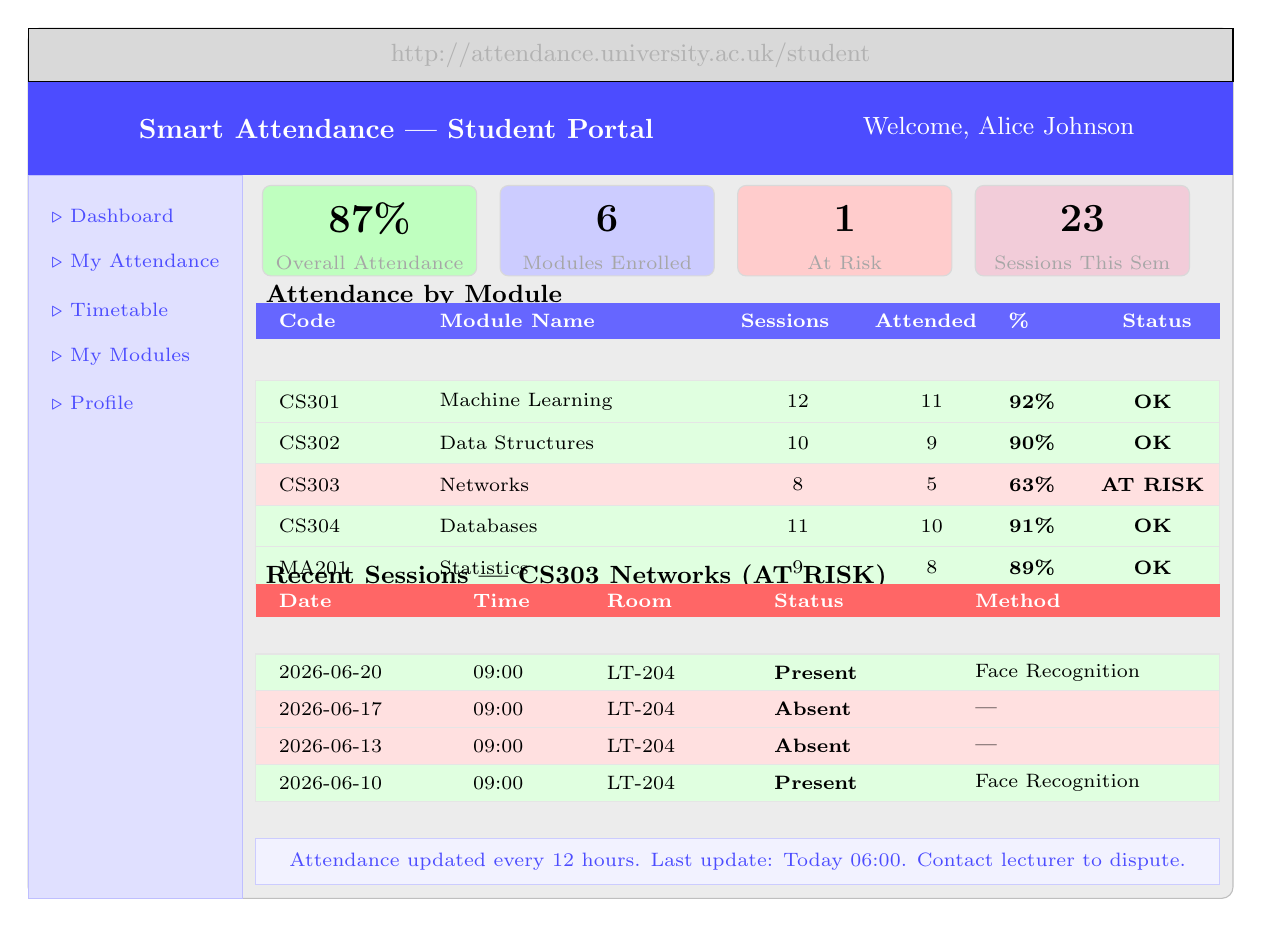
\begin{tikzpicture}[scale=0.85]

  \draw[fill=gray!15,draw=gray!50,rounded corners=4pt] (0,0) rectangle (18,13);
  \draw[fill=gray!30] (0,12.2) rectangle (18,13);
  \node[font=\small,text=gray!60] at (9,12.6) {http://attendance.university.ac.uk/student};

  % Header
  \draw[fill=blue!70,draw=none] (0,10.8) rectangle (18,12.2);
  \node[font=\bfseries,text=white] at (5.5,11.5) {Smart Attendance — Student Portal};
  \node[font=\small,text=white!80] at (14.5,11.5) {Welcome, Alice Johnson};

  % Sidebar
  \draw[fill=blue!12,draw=blue!25] (0,0) rectangle (3.2,10.8);
  \foreach \y/\lbl in {10.2/Dashboard,9.5/My Attendance,8.8/Timetable,8.1/My Modules,7.4/Profile}{
    \node[font=\scriptsize,text=blue!70,anchor=west] at (0.2,\y) {$\triangleright$\ \lbl};
  }

  % Stat cards
  \foreach \i/\val/\lbl/\col in {
    0/{87\%}/Overall Attendance/green!25,
    1/6/Modules Enrolled/blue!20,
    2/1/At Risk/red!20,
    3/23/Sessions This Sem/purple!20
  }{
    \pgfmathsetmacro{\xc}{3.5+\i*3.55}
    \draw[fill=\col,draw=gray!30,rounded corners=3pt]
      (\xc,9.3) rectangle (\xc+3.2,10.65);
    \node[font=\Large\bfseries] at (\xc+1.6,10.15) {\val};
    \node[font=\scriptsize,text=gray!70] at (\xc+1.6,9.5) {\lbl};
  }

  % Module table
  \node[font=\small\bfseries,anchor=west] at (3.4,9.0) {Attendance by Module};
  \draw[fill=blue!60,draw=none] (3.4,8.35) rectangle (17.8,8.9);
  \foreach \x/\hdr in {3.6/Code,6.0/Module Name,10.5/Sessions,12.5/Attended,14.5/\%,16.2/Status}{
    \node[font=\scriptsize\bfseries,text=white,anchor=west] at (\x,8.63) {\hdr};
  }
  \foreach \i/\code/\name/\s/\a/\pct/\col/\st in {
    0/CS301/{Machine Learning}/12/11/{92\%}/green!12/OK,
    1/CS302/{Data Structures}/10/9/{90\%}/green!12/OK,
    2/CS303/Networks/8/5/{63\%}/red!12/{AT RISK},
    3/CS304/Databases/11/10/{91\%}/green!12/OK,
    4/MA201/Statistics/9/8/{89\%}/green!12/OK
  }{
    \pgfmathsetmacro{\ytop}{8.35-\i*0.62-0.62}
    \pgfmathsetmacro{\ybot}{8.35-\i*0.62-1.24}
    \pgfmathsetmacro{\ymid}{(\ytop+\ybot)/2}
    \draw[fill=\col,draw=gray!20] (3.4,\ybot) rectangle (17.8,\ytop);
    \node[font=\scriptsize,anchor=west] at (3.6,\ymid) {\code};
    \node[font=\scriptsize,anchor=west] at (6.0,\ymid) {\name};
    \node[font=\scriptsize] at (11.5,\ymid) {\s};
    \node[font=\scriptsize] at (13.5,\ymid) {\a};
    \node[font=\scriptsize\bfseries] at (15.0,\ymid) {\pct};
    \node[font=\scriptsize\bfseries] at (16.8,\ymid) {\st};
  }

  % Recent sessions
  \node[font=\small\bfseries,anchor=west] at (3.4,4.8) {Recent Sessions — CS303 Networks (AT RISK)};
  \draw[fill=red!60,draw=none] (3.4,4.2) rectangle (17.8,4.7);
  \foreach \x/\hdr in {3.6/Date,6.5/Time,8.5/Room,11.0/Status,14.0/Method}{
    \node[font=\scriptsize\bfseries,text=white,anchor=west] at (\x,4.45) {\hdr};
  }
  \foreach \i/\dt/\ti/\rm/\st/\col/\me in {
    0/{2026-06-20}/{09:00}/LT-204/Present/green!12/{Face Recognition},
    1/{2026-06-17}/{09:00}/LT-204/Absent/red!12/{---},
    2/{2026-06-13}/{09:00}/LT-204/Absent/red!12/{---},
    3/{2026-06-10}/{09:00}/LT-204/Present/green!12/{Face Recognition}
  }{
    \pgfmathsetmacro{\ytop}{4.2-\i*0.55-0.55}
    \pgfmathsetmacro{\ybot}{4.2-\i*0.55-1.1}
    \pgfmathsetmacro{\ymid}{(\ytop+\ybot)/2}
    \draw[fill=\col,draw=gray!20] (3.4,\ybot) rectangle (17.8,\ytop);
    \node[font=\scriptsize,anchor=west] at (3.6,\ymid) {\dt};
    \node[font=\scriptsize,anchor=west] at (6.5,\ymid) {\ti};
    \node[font=\scriptsize,anchor=west] at (8.5,\ymid) {\rm};
    \node[font=\scriptsize\bfseries,anchor=west] at (11.0,\ymid) {\st};
    \node[font=\scriptsize,anchor=west] at (14.0,\ymid) {\me};
  }

  % Footer
  \draw[fill=blue!5,draw=blue!20] (3.4,0.2) rectangle (17.8,0.9);
  \node[font=\scriptsize,text=blue!70] at (10.6,0.55) {Attendance updated every 12 hours. Last update: Today 06:00. Contact lecturer to dispute.};

\end{tikzpicture}

\end{document}
